\documentclass[simplex.tex]{subfiles}
% NO NEED TO INPUT PREAMBLES HERE
% packages are inherited; you can compile this on its own
\begin{document}
\subsection{Non-Parametric Shape Clustering}

Energy statistics provides a nonparametric test for equality of distributions.
It is rotational invariant which is a highly desirable quality
for clustering. For a two-class problem, $X,X' \sim \mu$ and 
$Y,Y' \sim \nu$, where $\mu,\nu$ are CDFs, it reads
\begin{equation}\label{eq:energy}
\mathcal{E}(X,Y) = 2\mathbb{E} \| X - Y \|
- \mathbb{E} \| X - X' \| - \mathbb{E} \| Y - Y'\|.
\end{equation}
We are developing a clustering framework based on \ref{eq:energy}.
Our criteria is that $\mathcal{E}$ should be a maximum when data points are
correctly classified.
%
It is possible to show that there is a map from the data space of $X,Y$
to the probability space of $\mu,\nu$ which is a Hilbert space whose
inner product  can be obtained from a kernel 
function related to \ref{eq:energy}, 
$\langle \mu, \nu \rangle
= k(x,y)$.
This enables us to formulate our clustering problem as follows:
\begin{equation}\label{eq:opt}
\textnormal{max} \left\{ \textnormal{Tr} L^{1/2} Z^T K Z L^{1/2} \right\}
\quad
\textnormal{s.t.} \quad 
\, Z_{ij}\in\{0,1\}, \sum_i Z_{ij} = N_j, \sum_j Z_{ij}=1,
Z^T Z = L^{-1}
\end{equation}
where $N_j$ is the number of elements in the $j$th cluster,
$L^{-1}=\textnormal{diag}(N_1,\dotsc,N_k)$, and $K$ is the Gram 
matrix obtained
from the kernel. Let $\mathcal{X}$ be the pooled data matrix. If we
replace $K \to \mathcal{X}^T \mathcal{X}$ we recover the well-known
$k$-means problem, which in this formulation is related
to spectral clustering and normalized cuts. Problem
\ref{eq:opt} is 
NP-hard and a numerical implementation is prohibitive even
for small data sets. We are investigating how to 
solve \ref{eq:opt} in
a feasible way. As an evidence that \ref{eq:opt} is the correct optimization
problem, and more importantly, it illustrates the power behind our proposal,
in Fig.~\ref{fig:plots} we generate data and plot the objective in 
\ref{eq:opt} versus $n$, where $n$ is the number of points randomly shuffled
from one class to the other. Therefore, for $n=0$ the function must be a
maximum. We do this for the kernel related to \ref{eq:energy} (blue dots)
and compare with the kernel related to $k$-means (red dots).
Clearly, \ref{eq:opt} based on \ref{eq:energy} is able to distinguish
between different cluster even for complex data sets that are
not linearly separable. Moreover, in our formulation
there are no free-parameters in the kernel.

\begin{figure}[h!]
\begin{cframed}
\centering
\begin{minipage}{0.49\textwidth}
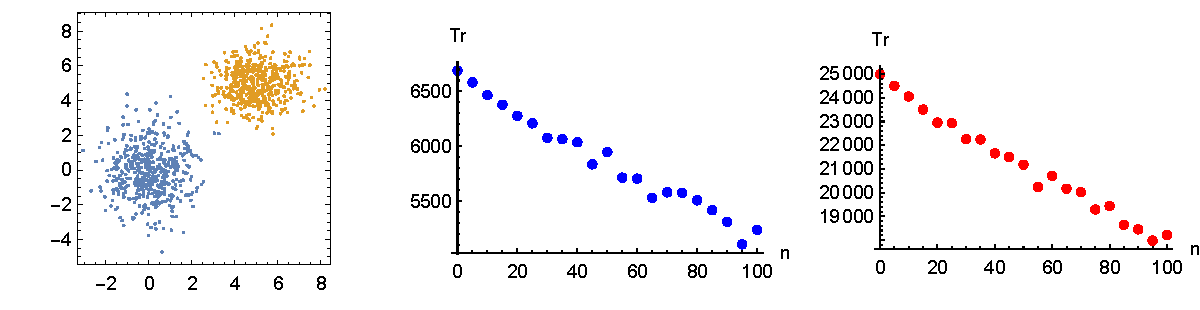
\includegraphics[scale=.37]{../../figs/plot1.pdf}
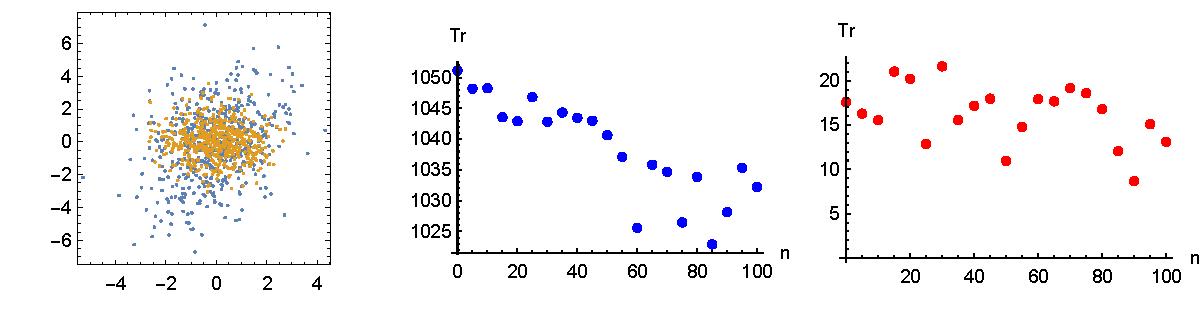
\includegraphics[scale=.37]{../../figs/plot2.pdf}
\end{minipage}
\begin{minipage}{0.49\textwidth}
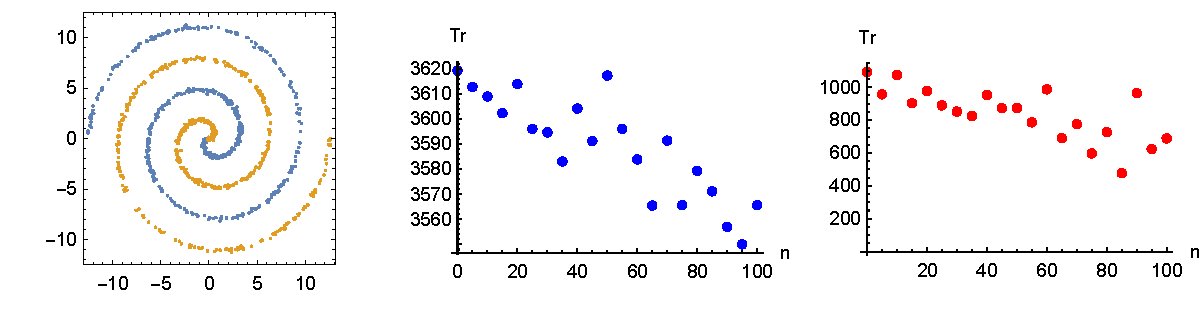
\includegraphics[scale=.37]{../../figs/plot3.pdf}
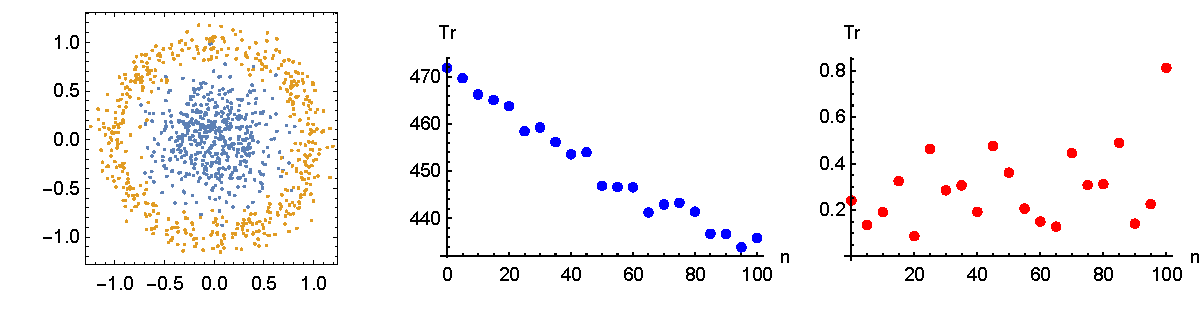
\includegraphics[scale=.37]{../../figs/plot4.pdf}
\end{minipage}
\caption{
Two dimensional datasets and the objective function
in \ref{eq:opt} as a function of $n$, where $n$ is the number of shuffled
points from its correct class to the wrong class. Blue dots
are for \ref{eq:energy} and red dots for $k$-means. A good function must
be monotonically decreasing. We can clearly see that \ref{eq:energy} is
way more powerful than $k$-means.
}
\label{fig:plots}
\end{cframed}
\end{figure}
%%
%\clearpage
\end{document}
